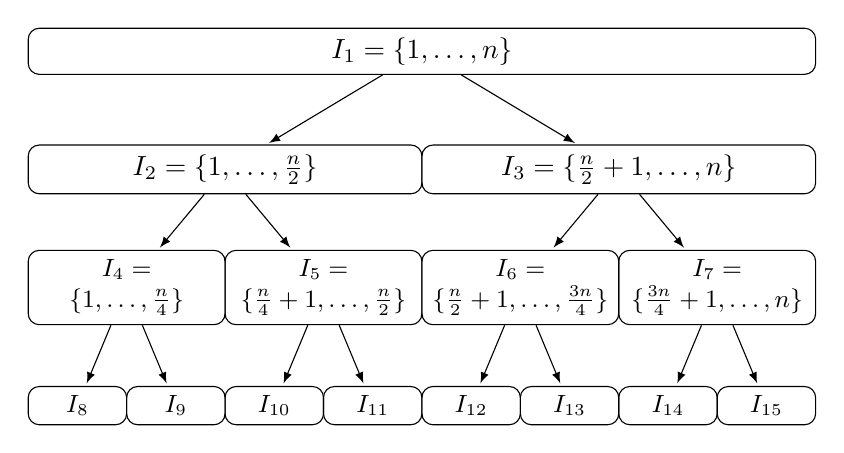
\begin{tikzpicture}[shorten >=1pt,
    edge from parent/.style={draw,-latex},
    level 1/.style={sibling distance=5cm, minimum width=5cm},
    level 2/.style={sibling distance=2.5cm, minimum width=2.5cm,font=\small},
    level 3/.style={sibling distance=1.25cm, minimum width=1.25cm},
    every node/.style = {shape=rectangle, rounded corners,
    draw, align=center}]
    \node[minimum width=10cm](I1){$I_1 = \{1, \ldots, n\}$}
    child {node{$I_2 = \{1, \ldots, \frac{n}{2}\}$}
        child{node{$I_4=$\\$\{1, \ldots, \frac{n}{4}\}$}
            child{node{$I_8$}}
            child{node{$I_9$}}
        }
        child{node{$I_5=$\\$\{\frac{n}{4}+1, \ldots, \frac{n}{2}\}$}
            child{node{$I_{10}$}}
            child{node{$I_{11}$}}
        }
    }
    child {node{$I_3 = \{\frac{n}{2}+1, \ldots, n\}$}
        child{node{$I_6=$\\$\{\frac{n}{2}+1, \ldots, \frac{3n}{4}\}$}
            child{node{$I_{12}$}}
            child{node{$I_{13}$}}
        }
        child{node{$I_7=$\\$\{ \frac{3n}{4}+1, \ldots, n\}$}
            child{node{$I_{14}$}}
            child{node{$I_{15}$}}
        }
    }
    ;
\end{tikzpicture}
